\section{Monopolie}
\todo[inline]{TODO: Waarom MO de helft van V?}
=\'e\'en aanbieder aanwezig zonder goede substituten voor zijn product. Monopolist wordt dus als enige geconfronteerd met de marktvraag. $\Rightarrow$ monopolist heeft marktmacht en is \textbf{prijszetter} (binnen bepaalde marges). Bijgevolg is de ondernemingsvraag = marktvraag. Monopolist zal dus moeten kiezen, hogere $p$ bij lagere $q$ of omgekeerd. De keuze hangt af van $\varepsilon^V_p$.

\subsection{Winstmaximalisatie bij Monopolie}
Een monopolist zal, net zoals elke andere ondernemer, proberen zijn winst te maximaliseren. Net zoals anders is dat als aan volgende voorwaarden voldaan zijn:
\begin{align}
   MO(q^*) &= MK(q^*) \\
   p \ge GK_{LT}(q^*) &\text{ of } p \ge GVK_{KT}(q^*)
\end{align}
Hij gaat echter niet de prijs vragen die bij dit punt hoort, maar de marginale bereidheid tot betalen ($V$) voor de bijhorende $q$ in dat punt. Er ontstaat dus een soort \textbf{markup ($\mu$)} boven op de normaal gevraagde prijs. Deze markup is de afstand tussen de $p$ in het punt waar $MO = MK$ en het punt op de vraagrechte voor de zelfde $q$ als dat evenwicht zoals je kan zien in figuur~\ref{fig:globaleMarktEnAanbodEenProducent}.

\begin{figure}[htbp]
   \centering
   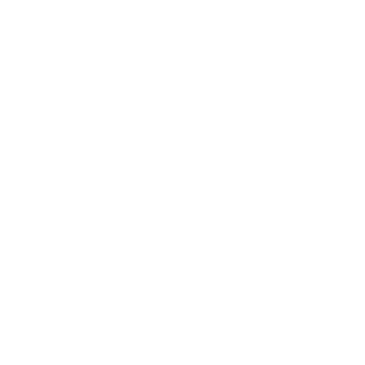
\includegraphics[scale=0.4]{Images/white.png}
   \caption{Winstmaximalisatie voor een monopolist (slide 6)}
   \label{fig:globaleMarktEnAanbodEenProducent}
\end{figure}

Zie slide 8 waarom $MO$ mooi onder $V$ ligt en de x-as zal snijden in het punt waar $\varepsilon^V_p = -1$. Dit wil wel zeggen dat een monopolist steeds op het elastische deel van de vraagcurve zal produceren, namelijk:
\begin{equation}
   \mu = p - MK = p - MO = \frac{p}{|\varepsilon^V_p|}
\end{equation}


\subsection{Prijsdiscriminatie}
Prijsdiscriminatie gaat over het vragen van verschillende prijzen aan verschillende doelgroepen voor hetzelfde product. Figuur~\ref{fig:perfectePrijsDiscriminatie} geeft een irre\"eel voorbeeld. Hier kan de aanbieder namelijk aan elk individu een andere prijs aanrekenen zo dat:
\begin{itemize}
   \item elk individu betaalt wat hij bereid is te betalen
   \item opbrengsten nemen toe met het consumentensurplus
\end{itemize}
Het ganse consumentensurplus wordt dus ``afgeroomd''. De monopolist zal nu ook meer willen produceren, tot het punt waar $MO = p \text{ (=vraagcurve)}$, om ook dat laatste stukje consumentensurplus te kunnen afromen.
\begin{figure}[htbp]
   \centering
   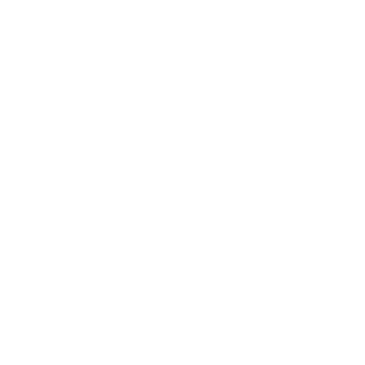
\includegraphics[scale=0.4]{Images/white.png}
   \caption{Perfecte prijsdiscriminatie (slide 12)}
   \label{fig:perfectePrijsDiscriminatie}
\end{figure}

Het is echter zo dat de bereidheid tot betalen niet te observeren valt $\Rightarrow$ onrealistische situatie.

Er zijn twee vormen die wel voorkomen:
\begin{description}
   \item[Marktsegmentatie]: De monopolist gaat de consument in groepen opdelen
   \item[Zelfselectie]: er worden drempels ingebouwd waardoor consumenten met een verschillende bereidheid tot betalen zichzelf indelen in verschillende groepen.
\end{description}

Bij marktsegmentatie zullen consumenten met een hogere $\varepsilon^V_p$ een lagere prijs krijgen (figuur~\ref{fig:marktsegmentatie}). In elke deelmarkt zal $q^*$ worden aangeboden die tot stand komt door het zoeken waar $MO = MK$, maar dit zal in de twee deelgroepen leiden tot een andere prijs.
\begin{figure}[htbp]
   \centering
   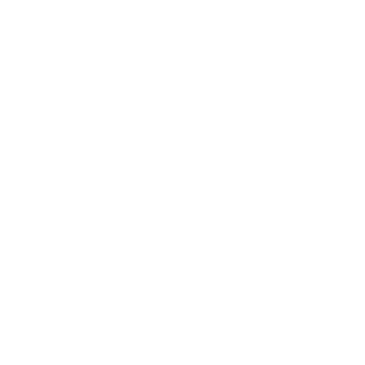
\includegraphics[scale=0.4]{Images/white.png}
   \caption{Prijsdiscriminatie via marktsegmentatie (slide 14)}
   \label{fig:marktsegmentatie}
\end{figure}

Er zijn tevens 2 voorwaarden opdat je aan marktsegmentatie zou kunnen doen:
\begin{itemize}
   \item Er moet een duidelijk onderscheid gemaakt kunnen worden tussen de verschillende groepen
   \item Je moet kunnen verhinderen dat mensen van de groep met de hoge prijs zich kunnen voordoen als iemand van de groep met de lagere prijs
\end{itemize}

Zelfselectie gaat iets anders te werk. Een goed voor beeld is diesel- $><$ benzinewagens. Vanaf een bepaald aantal gereden kilometer is het goedkoper om een dieselwagen te kopen $\Rightarrow$ mensen die veel rijden kopen toch een duurdere dieselwagen, ook al is die niet duurder om te produceren.

Een vorm van zelfselectie is \textbf{intertemporele tijdsdiscriminatie}. Vakantiehuizen kunnen hier als voorbeeld dienen. Deze zijn namelijk durder in het hoogseizoen en in verlengde weekends $\Rightarrow$ wie meer geld heeft kan gaan wanneer het duurder is en moet bvb. geen extra vakantiedag opgeven om op een ander moment een lang weekend weg te gaan.


\subsection{Oorzaken van Monopolie}
Een monopolie kan enkel blijven bestaan mits er toetredingsbelemmeringen zijn:
\begin{itemize}
   \item Technologische belemmeringen:
      \begin{itemize}
         \item schaalvoordelen en \textbf{natuurlijke monopolies}. Dit komt voor wanneer het minimum van $GK/GVK$ zich pas bij een zeer hoge $q*$ voordoet $\Rightarrow$ er zal enkel plaats zijn voor 1 onderneming. Indien er een paar ondernemingen zijn, zal de grootste de laagste $GK$ hebben en dus op ``natuurlijke wijze'' de anderen wegconcurreren.
         \item exclusief gebruiksrecht van productiefactoren.
         \item technologische kennis: je bent de enige dat iets specifiek weet
      \end{itemize}
   \item Wettelijke belemmeringen
      \begin{itemize}
         \item concurrentieverbod: vaak worden deze ondernemingen dan wel gecontroleerd door de overheid en zal hun marktmacht (=markup) aan banden worden gelegd
         \item beperkte licenties: bvb telecom, apotheken
         \item tijdelijke monopolies door patenten
      \end{itemize}
   \item Strategisch gedrag: dreigen met dure rechtzaken/marketingcampagnes
\end{itemize}
\subsection{Welvaartsanalyse van Monopolie}
Waar in de markt bij vrije mededinging het evenwicht tot stand kwam waar $V=A$($=MK$), zal dat bij monopolie niet zo zijn. Hij zal produceren in het punt $MO=MK$ en dan de bijhorende prijs op de vraagcurve voor die hoeveelheid vragen en er zal ``een driehoekje'' van welvaart verloren gaan.

$p=MK(q^*)$ geldt niet meer en pareto-effici\"entie is dus niet bereikt. Nu geldt namelijk dat $p>MK(q^*)$ en indien er meer geproduceerd zou worden, is er zeker iemand die meer wil betalen dan wat het zou kosten om deze extra eenheid te produceren.

De vraag of de overheid hier iets aan doen werpt zich dan op. Kan ze dit welvaarsverlies verkleinen of zelfs helemaal elimineren? Een eerste idee kan zijn om de monopolist te belasten met bvb. een accijns (figuur~\ref{fig:belastingOpMonopolist}). Zoals je kan zien zal dit echter inhouden dat de monopolist net minder en tegen een hogere $p$ zal gaan produceren, wat net het omgekeerde is van wat we willen bereiken.
\begin{figure}[htbp]
   \centering
   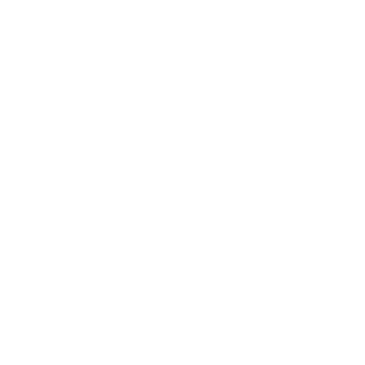
\includegraphics[scale=0.4]{Images/white.png}
   \caption{Belasting op monopolist (slide 21)}
   \label{fig:belastingOpMonopolist}
\end{figure}

Stel dat er een proportionele winstbelasting wordt ingevoerd. Dit zal geen effect hebben op het gedrag van de monopolist. De winst zal in elk punt gewoon evenredig afnemen, maar de optimale $q^*$ zal dezelfde blijven.

Een maximumprijs is een andere mogenlijkheid. Zoals je in figuur~\ref{fig:GOMOmonopolistBijMaximumprijs} kan zien, zullen na de introductie van een maximumprijs $MO$ en $GO$ gelijk zijn aan die maximumprijs tot in het punt waar $p_{MAX} = GO$ (=vraagcurve). Na dat punt zijn ze beide terug gelijk aan hun oude curve.

\begin{figure}[htbp]
   \centering
   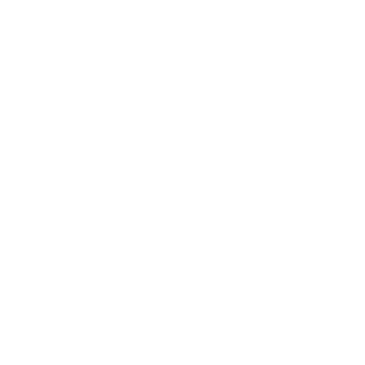
\includegraphics[scale=0.4]{Images/white.png}
   \caption{MO en GO monopolist bij maximumprijs (slide 24 \& 25)}
   \label{fig:GOMOmonopolistBijMaximumprijs}
\end{figure}

Als we dan ook nog $MK$ en $GK$ invoeren om het optimum te vinden, lijkt het op het eerste zicht dat er geen punt meer is waar $MO = MK$. Het optimum zal echter in het \textbf{scharnierpunt} van $GO$ liggen. Het is in dat punt namelijk zo dat:
\begin{itemize}
   \item in een kleinere $q$: $MO > MK$
   \item in een grotere $q$: $MO < MK$
\end{itemize}
Bijgevolg is het scharnierpunt optimaal.

We kunnen nu inzien dat er een maximumprijs bestaat waarvoor geldt dat het welvaartsverlies volledig teniet gedaan wordt, namelijk wanneer $p_{MAX}$ gelijk is aan de $p$ die hoort bij het punt waar $MK = V$. In de praktijk is dit punt echter moeilijk te vinden.

Een uitzondering hierop ontstaat bij \textbf{natuurlijke monopolies} zoals je kan zien in figuur~\ref{fig:maximumprijsNatuurlijkMonopolie}. Een maximumprijs die ervoor zorgt dat het evenwicht ligt in $MK = V$ kan ervoor zorgen dat de monopolist verlies maakt en dus uit de markt zou treden. Om dit tegen te gaan moet de overheid ofwel het verlies met subsidies compenseren, of een maximumprijs opleggen zodat $GK = V$ en de monopolist dus bread-even draait.
\begin{figure}[htbp]
   \centering
   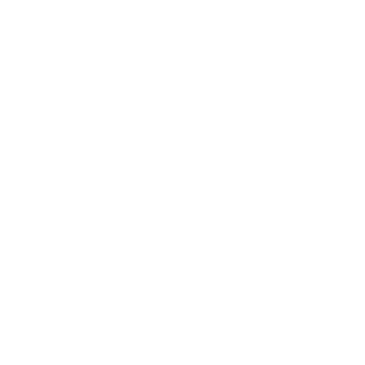
\includegraphics[scale=0.4]{Images/white.png}
   \caption{Maximumprijs bij natuurlijk monopolie (slide 32)}
   \label{fig:maximumprijsNatuurlijkMonopolie}
\end{figure}
